% !TeX root = main.tex
\documentclass{article}
%\usepackage{blindtext}
%\usepackage[a4paper, total={6in, 9.4in}]{geometry}

% % \documentclass[a4paper,14pt, draft]{article}

%%% отключение нумерации сраниц
\pagestyle{empty}
%%% значок в itemize
% \renewcommand{\labelitemi}{$\cdot$}

%%% Работа с русским языком
\usepackage{cmap}					% поиск в PDF
\usepackage{mathtext} 				% русские буквы в формулах
\usepackage[T1, T2A]{fontenc}			% кодировка %Т1 посоветовал чат гпт
\usepackage[utf8]{inputenc}			% кодировка исходного текста
\usepackage[english,russian]{babel}	% локализация и переносы
\usepackage{indentfirst}            % красная строка в первом абзаце
\frenchspacing                      % равные пробелы между словами и предложениями

%%% Дополнительная работа с математикой
\usepackage{amsmath,amsfonts,amssymb,amsthm,mathtools} % пакеты AMS
\usepackage{icomma}                                    % "Умная" запятая

%%% Свои символы и команды
\usepackage{centernot} % центрированное зачеркивание символа
\usepackage{stmaryrd}  % некоторые спецсимволы
\usepackage{dsfont}
\usepackage{amsthm}


\renewcommand{\epsilon}{\ensuremath{\varepsilon}}
\renewcommand{\phi}{\ensuremath{\varphi}}
\renewcommand{\kappa}{\ensuremath{\varkappa}}
\renewcommand{\le}{\ensuremath{\leqslant}}
\renewcommand{\leq}{\ensuremath{\leqslant}}
\renewcommand{\ge}{\ensuremath{\geqslant}}
\renewcommand{\geq}{\ensuremath{\geqslant}}
\renewcommand{\emptyset}{\ensuremath{\varnothing}}

\DeclareMathOperator{\sgn}{sgn}
\DeclareMathOperator{\ke}{Ker}
\DeclareMathOperator{\im}{Im}
\DeclareMathOperator{\re}{Re}

\newcommand{\N}{\mathbb{N}}
\newcommand{\Z}{\mathbb{Z}}
\newcommand{\Q}{\mathbb{Q}}
\newcommand{\R}{\mathbb{R}}
\newcommand{\Cm}{\mathbb{C}}
\newcommand{\F}{\mathbb{F}}
\newcommand{\id}{\mathrm{id}}
\newcommand{\imp}[2]{
	(#1\,\,$\ra$\,\,#2)\,\,
}
\newcommand{\Root}[2]{
	\left\{\!\sqrt[#1]{#2}\right\}
}
\newcommand{\RR}{\R}
\newcommand{\NN}{\N}
\renewcommand{\subseteq}{\subset}
\newcommand{\sub}{\subset}
\newcommand{\sconstr}{\;\vert\;}
\newcommand{\thus}{\implies}

\newcommand{\defeq}{\vcentcolon= }
\newcommand{\defev}{\stackrel{\Delta}{\Longleftrightarrow}}
\newcommand{\deriv}[3][1]{%
	\ifthenelse{#1>1}{%
		\frac{\dlta^{#1} {#2}}{\dlta {#3}^{#1}}
	}{%
		\frac{\dlta {#2}}{\dlta {#3}}
	}%
}

\renewcommand\labelitemi{$\triangleright$}

\let\bs\backslash
\let\lra\Leftrightarrow
\let\ra\Rightarrow
\let\la\Leftarrow
\let\emb\hookrightarrow

%%% Перенос знаков в формулах (по Львовскому)
\newcommand{\hm}[1]{#1\nobreak\discretionary{}{\hbox{$\mathsurround=0pt #1$}}{}}

%%% Работа с картинками
\usepackage{graphicx}    % Для вставки рисунков
\setlength\fboxsep{3pt}  % Отступ рамки \fbox{} от рисунка
\setlength\fboxrule{1pt} % Толщина линий рамки \fbox{}
\usepackage{wrapfig}     % Обтекание рисунков текстом

% \usepackage[inkscapeformat=png]{svg} %% svg

%%% Работа с таблицами
\usepackage{array,tabularx,tabulary,booktabs} % Дополнительная работа с таблицами
\usepackage{longtable}                        % Длинные таблицы
\usepackage{multirow}                         % Слияние строк в таблице

%%% Теоремы
\theoremstyle{plain}
\newtheorem*{theorem}{Теорема}
\newtheorem*{lemma}{Лемма}
\newtheorem*{proposition}{Утверждение}
\newtheorem*{exercise}{Упражнение}
\newtheorem*{problem}{Задача}

\theoremstyle{definition}
\newtheorem*{definition}{Определение}
\newtheorem*{corollary}{Следствие}
\newtheorem*{note}{Замечание}
\newtheorem*{reminder}{Напоминание}
\newtheorem*{example}{Пример}

\theoremstyle{remark}
\newtheorem*{solution}{Решение}

%%% Оформление страницы
\usepackage{extsizes}     % Возможность сделать 14-й шрифт
\usepackage{geometry}     % Простой способ задавать поля
\usepackage{setspace}     % Интерлиньяж
\usepackage{enumitem}     % Настройка окружений itemize и enumerate
\setlist{leftmargin=10pt} % Отступы в itemize и enumerate

\geometry{top=15mm}    % Поля сверху страницы
\geometry{bottom=5mm} % Поля снизу страницы
\geometry{left=10mm}   % Поля слева страницы
\geometry{right=10mm}  % Поля справа страницы

\setlength\parindent{15pt}        % Устанавливает длину красной строки 15pt
\linespread{1}                  % Коэффициент межстрочного интервала
%\setlength{\parskip}{0.5em}      % Вертикальный интервал между абзацами
\setcounter{secnumdepth}{0}      % Отключение нумерации разделов
%\setcounter{section}{-1}         % Нумерация секций с нуля
\usepackage{multicol}			  % Для текста в нескольких колонках
\usepackage{soulutf8}             % Модификаторы начертания
\mathtoolsset{showonlyrefs=true} % показывать номера формул только у тех, у которых есть ссылки по eqref
%%% Содержаниие
% \usepackage{tocloft}
% \tocloftpagestyle{main}
%\setlength{\cftsecnumwidth}{2.3em}
%\renewcommand{\cftsecdotsep}{1}
%\renewcommand{\cftsecpresnum}{\hfill}
%\renewcommand{\cftsecaftersnum}{\quad}

%%% Нумерация уравнений
\makeatletter
\def\eqref{\@ifstar\@eqref\@@eqref}
\def\@eqref#1{\textup{\tagform@{\ref*{#1}}}}
\def\@@eqref#1{\textup{\tagform@{\ref{#1}}}}
\makeatother                      % \eqref* без гиперссылки
\numberwithin{equation}{section}  % Нумерация вида (номер_секции).(номер_уравнения)
\mathtoolsset{showonlyrefs= true} % Номера только у формул с \eqref{} в тексте.

%%% Гиперссылки
\usepackage{hyperref}
\usepackage[usenames,dvipsnames,svgnames,table,rgb]{xcolor}
\hypersetup{
	unicode=true,            % русские буквы в раздела PDF
	colorlinks=true,       	 % Цветные ссылки вместо ссылок в рамках
	linkcolor=black!15!blue, % Внутренние ссылки
	citecolor=green,         % Ссылки на библиографию
	filecolor=magenta,       % Ссылки на файлы
	urlcolor=NavyBlue,       % Ссылки на URL
}

%%% Графика
\usepackage{tikz}        % Графический пакет tikz
\usepackage{tikz-cd}     % Коммутативные диаграммы
\usepackage{tkz-euclide} % Геометрия
\usepackage{stackengine} % Многострочные тексты в картинках
\usetikzlibrary{angles, babel, quotes}
\usepackage{wrapfig}
\usepackage{graphicx}
\usepackage{mathtext}
\usepackage{amsmath}
\usepackage{siunitx} % Required for alignment
\usepackage{subfigure}
\usepackage{multirow}
\usepackage{rotating}
\usepackage{afterpage}
\usepackage[T1,T2A]{fontenc}
\usepackage[russian]{babel}
\usepackage{caption}
\usepackage[arrowdel]{physics}
\usepackage{booktabs}
\usepackage{float}


% \graphicspath{{pictures/}}

\begin{document}
\title{\begin{center}Лабораторная работа №3.7.1\end{center}
	Скин-эффект в полом цилиндре}
\author{Александр Ляпин, Кирилл Нелюбин, Б05-207}
\date{\today}

	\maketitle
	\section*{Цель работы:} Исследование проникновения переменного магнитного поля в медный полый цилиндр
	
	\section*{Экспериментальная установка}
\begin{figure}[H]
	\center
  \includegraphics*[width=0.7\textwidth]{24_12_48.png}
  \caption*{Экспериментальная установка для изучения скин-эффекта}
\end{figure}
\begin{figure}[H]
	\center
  \includegraphics*[width=0.7\textwidth]{24_12_59.png}
  \caption*{Схема подключения RLC-метра}
\end{figure}

	\section*{Ход работы}
	
	Параметры нашей установки $2a = 45$ мм, $h=1.5$ мм. Проводимость порядка
	$\sigma \sim 5\cdot 10^7$ См/м. Получаем оценку для частоты, при которой
	глубина проникновения равна толщине стенок цилиндра $\nu_h = 2254$ Гц.
	
	\subsection*{Измерения амплитуд в области низких частот}
	В области низких частот толщина скин-слоя превосходит толщину образца $ \delta \gg h$  и из (\ref{eq:svyaz_poley}) получаем
	\begin{equation*}
		\left(\frac{|H_1|}{|H_0|}\right)^2 = (\xi_0\xi)^2 \approx \frac{1}{1+\left(\frac{ah}{\delta^2}\right)^2} = \frac{1}{1 + \left(\pi ah\nu\mu_0\sigma\right)^2}
	\end{equation*}
	Тогда: 
	\begin{equation*}
		\frac{1}{\xi^2}=\xi_0^2B^2\nu^2 + \xi_0^2 \text{, где } B=\pi a h \sigma \mu_0
		\label{eq:liniya_dlya_c}
	\end{equation*}
	\begin{figure}[h!]
		\centering
		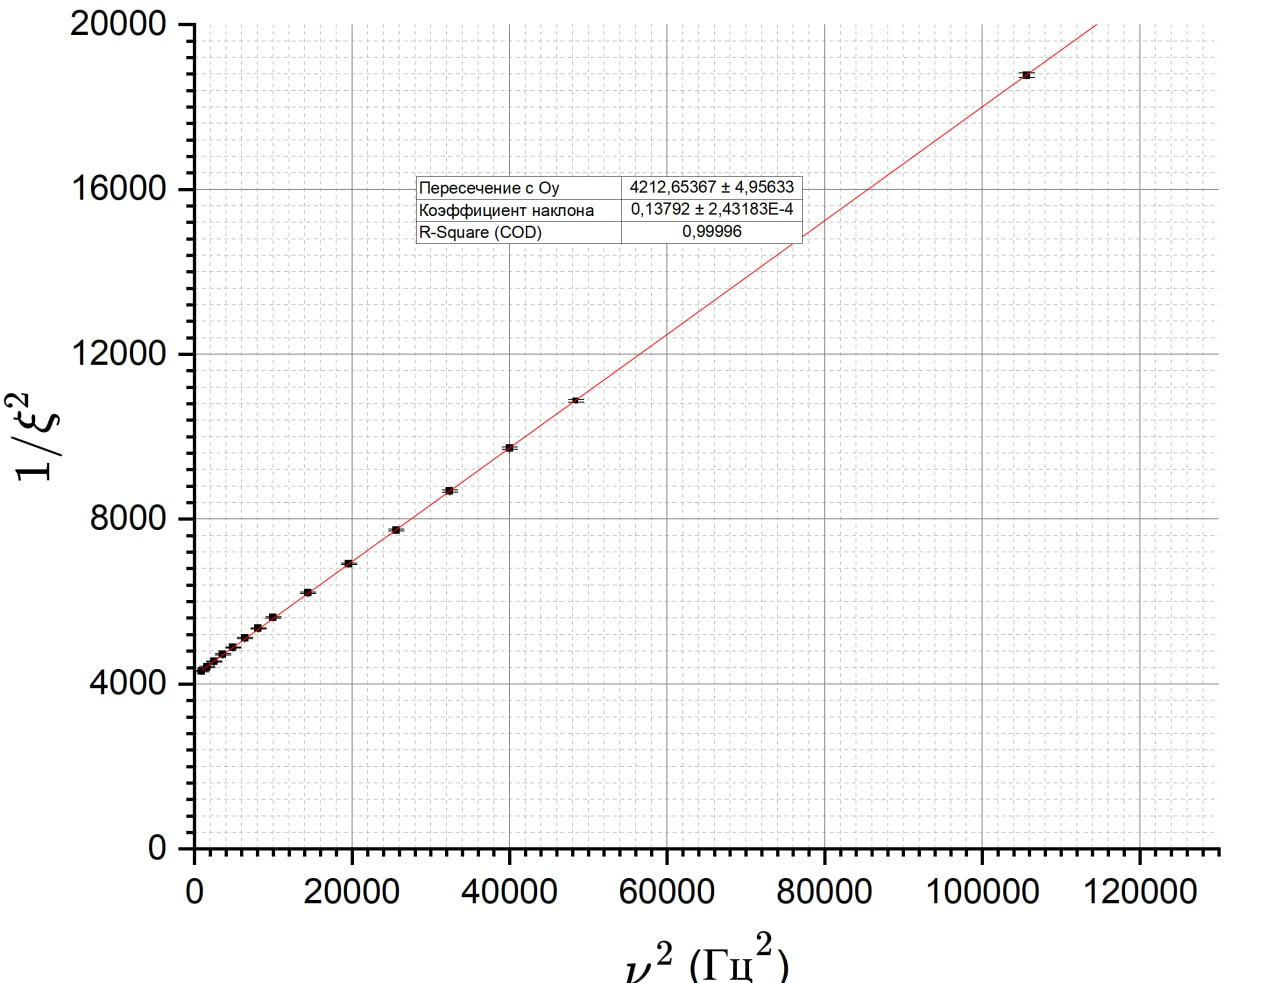
\includegraphics[width=0.9\textwidth, height = 0.45\textheight]{15_13_25.png}
		\caption{График зависимости $1/\xi^2(\nu^2)$}\label{fig:xi_nu_low_freq_linearized}
	\end{figure}
	Получаем следующие значения: $\xi_0^2B^2 = 0.138, \ \xi_0^2 = 4212.65$, тогда:
	\[\xi_0 = 64.90 \pm 0.04 \ \frac{\text{Гц}}{\text{Ом}}, \ \sigma = (4.294 \pm 0.005) \cdot 10^7 \ \frac{\text{См}}{\text{м}}  \]
	
	\subsection*{Измерение проводимости через разность фаз при низких частотах}
	Построим график $\tg{\psi} (\nu)$ по тем точкам точкам, для которых он хорошо аппроксимируется прямой (при $\nu \approx 0.5 \nu_h \ \tg \psi \rightarrow +\infty$) 
	Согласно формуле (\ref{eq:faza_low_freq}), при $\delta \gg h$
	\begin{equation*}
		\tg \psi = \frac{ahw \sigma \mu_0}{2} = \pi ah\mu_0\sigma \nu \ \ (\mu = 1)
	\end{equation*}
	Коэффициент наклона прямой: \[\pi ah \mu_0\sigma = k = (5.2 \pm 1) \cdot 10^{-3} \ \text{с}\]
	\[\sigma = \frac{k}{\pi ah \mu_0} = (3.93 \pm 0.73) \cdot 10^7 \ \frac{\text{См}}{\text{м}}\]
	\begin{figure}[H]
		\centering
		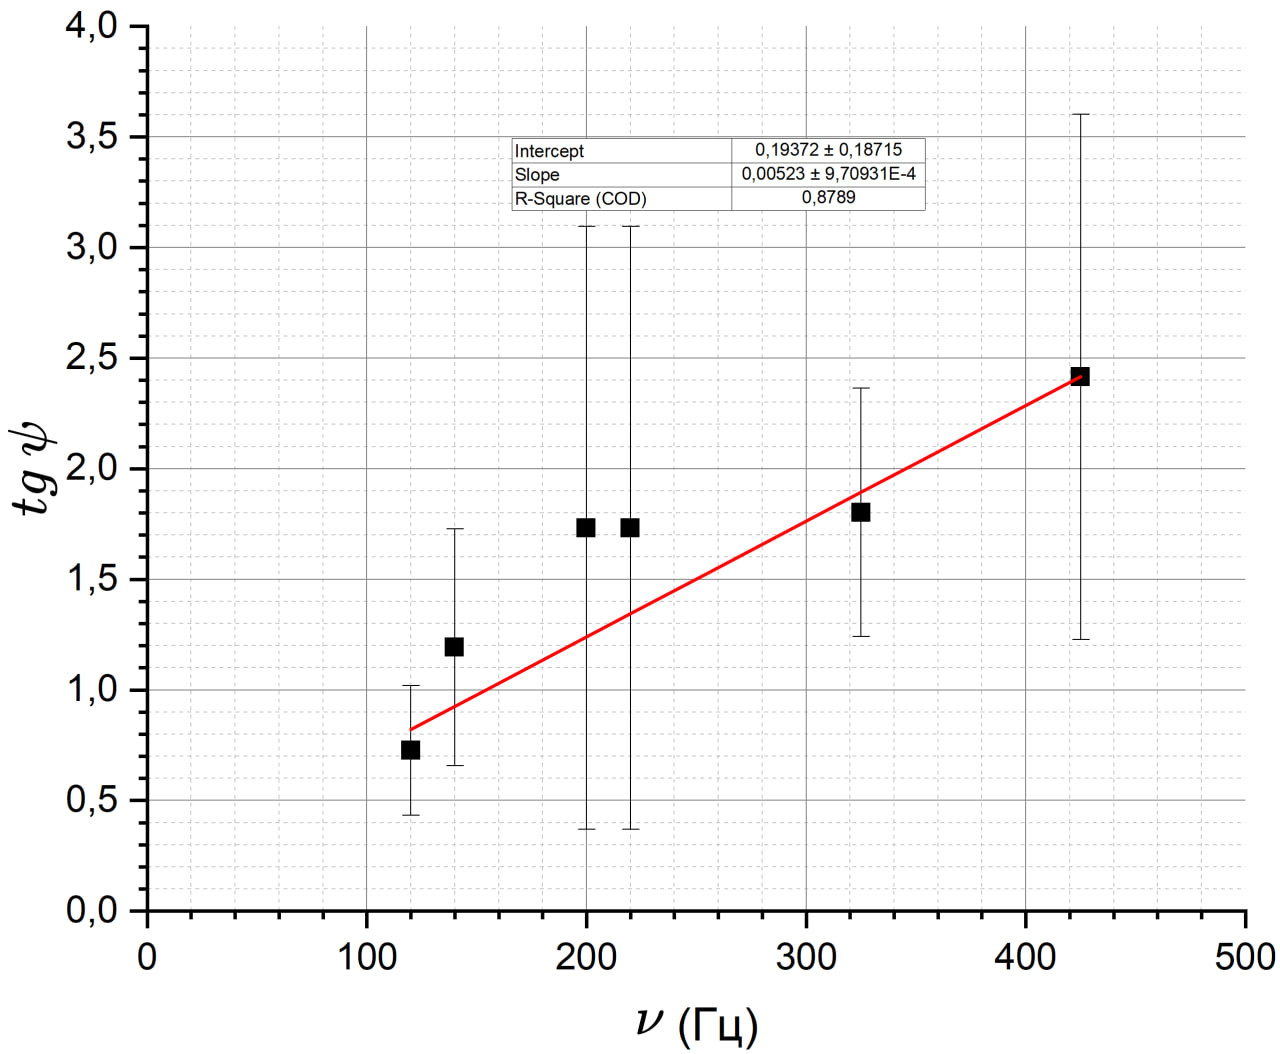
\includegraphics[width=0.7\textwidth]{15_13_28.png}
		\caption{График зависимости $\tg \psi (\nu)$}\label{fig:tg_psi_nu_line}
	\end{figure}

	\subsection*{Измерение проводимости через разность фаз в высокочастотном диапазоне}
	Согласно формуле (\ref{eq:faza_high_freq}), при $\delta \ll h$
	\begin{equation*}
		\psi - \pi/4 = k\cdot \sqrt{\nu}; \ k = h\sqrt{\pi\mu_0\sigma}
	\end{equation*}
	
	Получено значение $k = 0.0184 \pm 0.0014$, отсюда получаем значение проводимости:
	
	\begin{equation}
		\sigma = (3.80 \pm 0.58) \cdot 10^7 \ \frac{\text{См}}{\text{м}}
	\end{equation}
	
	\begin{figure}[h]
		\centering
		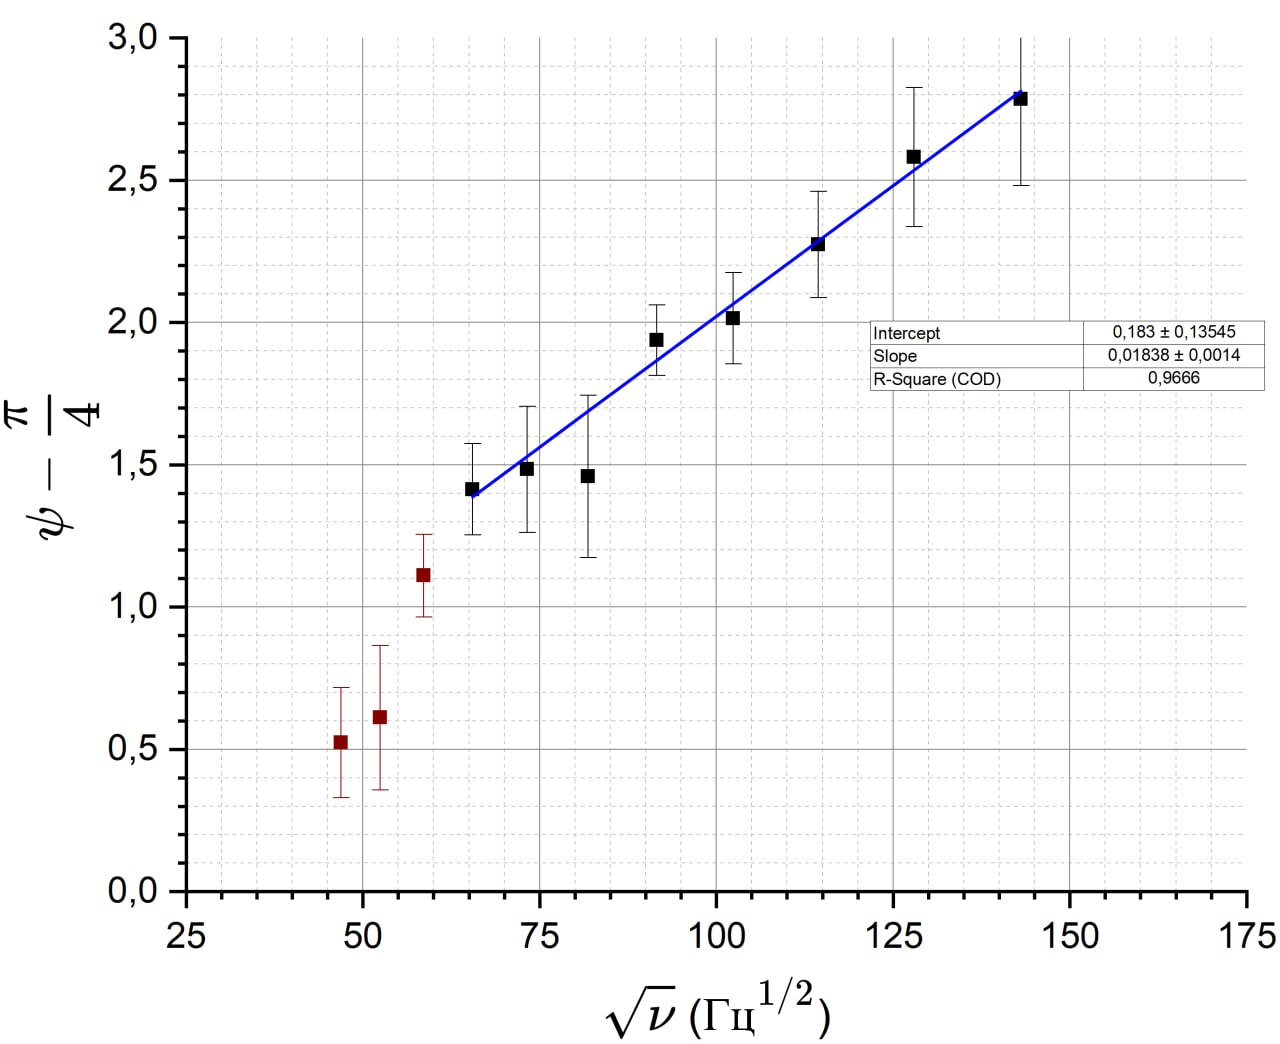
\includegraphics[width=\textwidth]{15_13_30.png}
		\caption{График зависимости $(\psi - \pi/4)(\sqrt{\nu})$}
		\newpage
	\end{figure}
	
	\subsection*{Измерение проводимости через изменение индуктивности}
	Измерить проводимость можно также через изменение индуктивности катушки внутри цилиндра. Данные, измеренные с помощью $RCL$-метра:
	
	\begin{table}[h!]
		\centering
		\begin{tabular}{|c|c|c|c|c|c|c|c|c|c|c|c|c|c|c|}
			\hline
			$\nu$, кГц & 0.04 & 0.15 & 0.25 & 0.3 & 0.4 & 0.5 & 0.6 & 0.8 & 1.5 & 2.5 & 4 & 10 & 15 & 20 \\
			\hline
			$L$, мГн & 10 & 7.35 & 5.4 & 4.8 & 4.0  & 3.65 & 3.45 & 3.26 & 2.9 & 2.9 & 2.9 & 3 & 3.17 & 3.6 \\
			\hline
		\end{tabular}
		\caption{Значения индуктивности катушки при различных частотах}
	\end{table}
	
	Примерно так выглядит график $L(\nu)$:
	
	\begin{figure}[H]
		\centering
		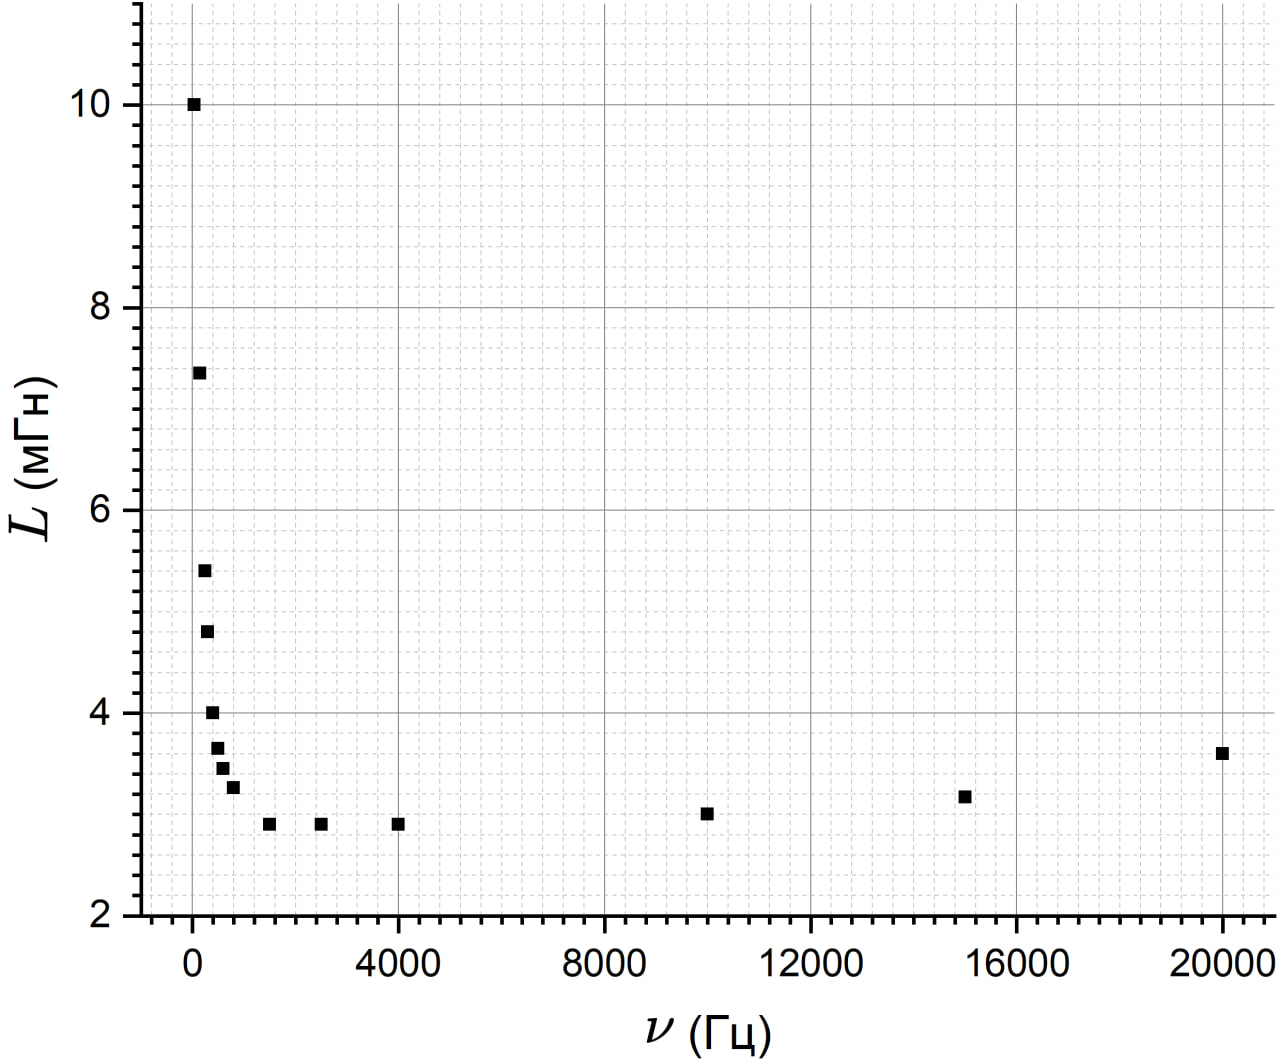
\includegraphics[width = 0.9\textwidth]{15_13_31.png}
		\caption{График зависимости $L(\nu)$}
	\end{figure}
	
	Полученные максимальные и минимальные значения: $L_{min} = 2.9$ мГн, $L_{max} = 10$ мГн.
	\begin{equation*}
		\frac{L_{\max} - L}{L - L_{\min}} = \pi ^2 a^2 h^2 {\mu_0}^2 \sigma^2 \nu^2
	\end{equation*}
	
	То есть коэффициент наклона графика
	\[k = (\pi ah\mu_0 \sigma)^2 \ \rightarrow \sigma = \frac{\sqrt{k}}{\pi ah \mu_0}\]
	
	Подставляя полученные значения, получаем:
	
	\begin{equation}
		\sigma = (4.11 \pm 0.07) \cdot 10^7  \ \frac{\text{См}}{\text{м}}
	\end{equation}
	
	\begin{figure}[h!]
		\centering
		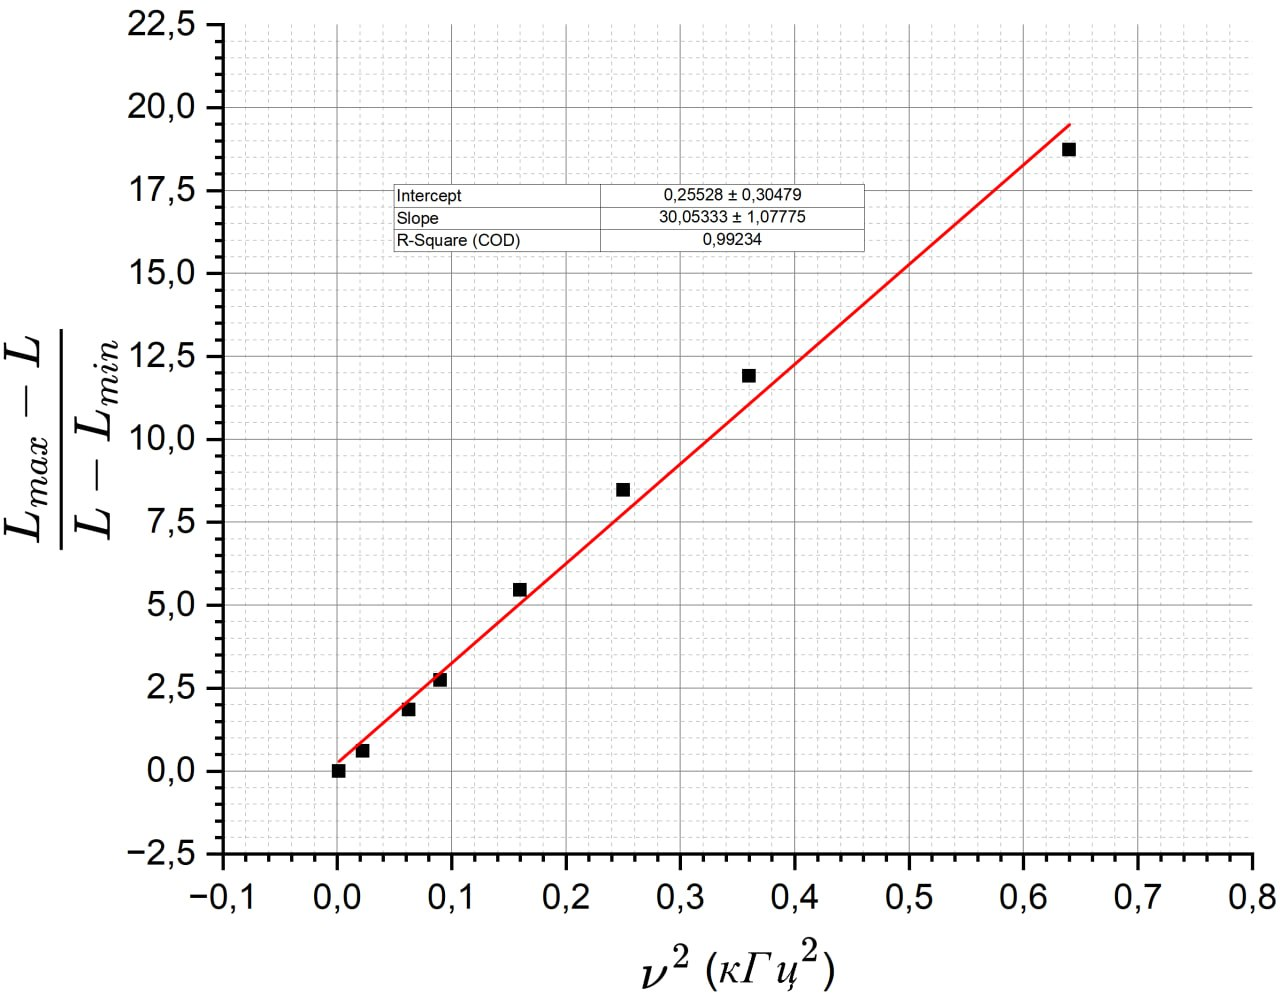
\includegraphics[width=\textwidth]{15_13_32.png}
		\caption{График зависимости $\frac{L_{\max} - L}{L - L_{\min}} (\nu^2)$}
	\end{figure}
	
	
	\subsection*{Отношение магнитных полей}
	Отношение $\abs{H_1}/\abs{H_0}$ можем посчитать двумя способами. Первый способ - через
	формулу (\ref{eq:otnoshenie_amplitud}),использовав посчитанное значение $\xi_0$ в анализе амплитуд в области низких частот.
	Второй способ - через теоретическую формулу (\ref{eq:svyaz_poley}), использовав первое полученное значение $\sigma$. Посмотрим на их различие с помощью графиков зависимости
	$\abs{H_1}/\abs{H_0} (\nu)$
	
	\begin{figure}[h]
		\centering
		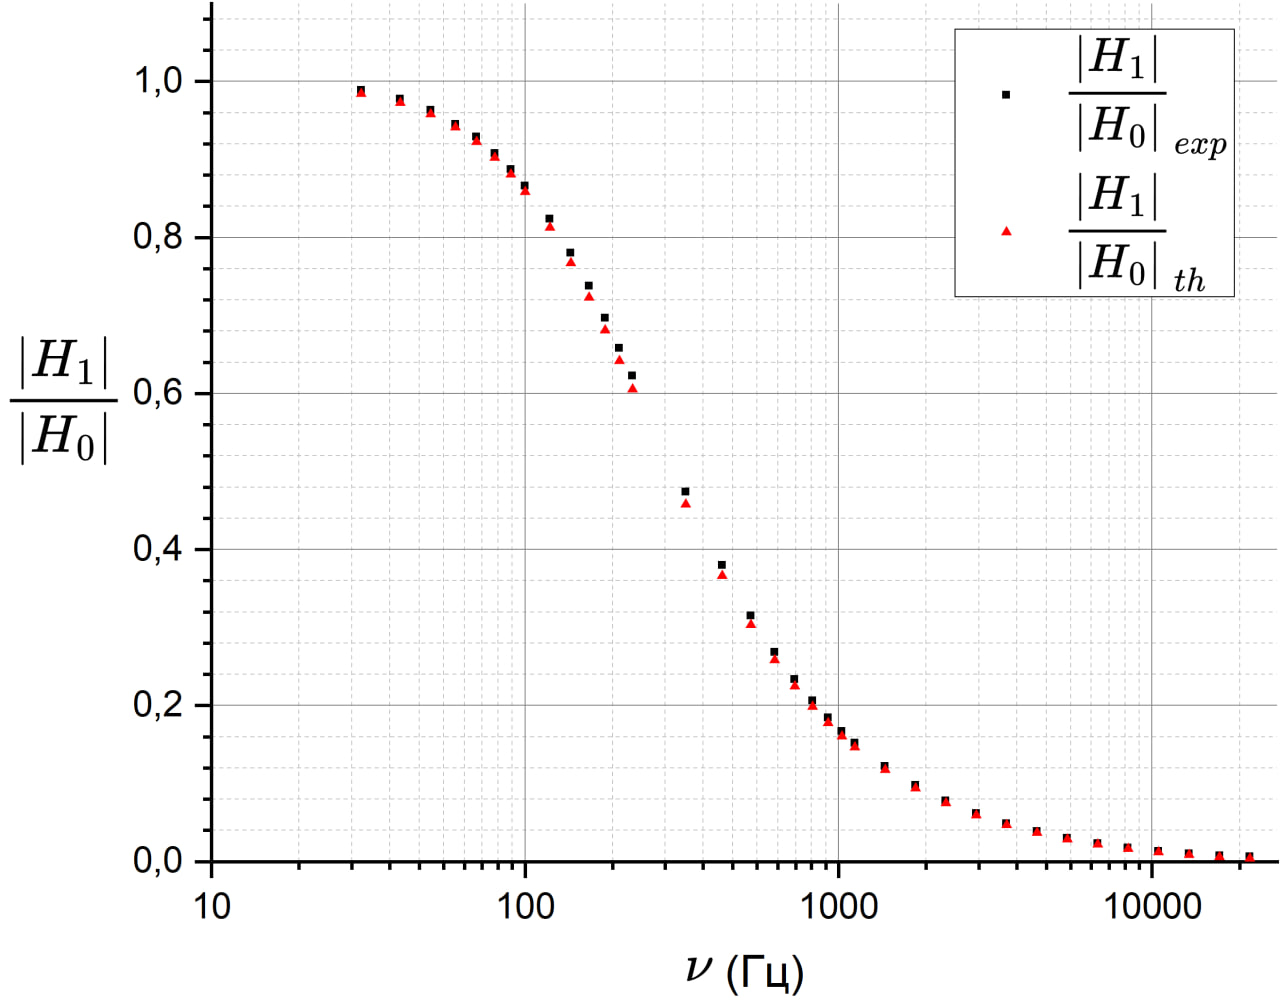
\includegraphics[width=\textwidth]{15_13_33.png}
		\caption{График зависимость $\frac{|H_1|}{|H_0|}(\nu)$}
	\end{figure}
	
	\section*{Выводы}
	В данной лабораторной работе мы измеряли удельную проводимость меди 4-мя различными способами с помощью явления скин-эффекта. Запишем результаты в общую таблицу:
	
	\begin{table}[!h]
		\begin{center}
			\begin{tabular}{|l|c|c|c|}
				\hline
				Метод измерения & $\sigma, 10^{7} \ \frac{\text{См}}{\text{м}}$ & $\Delta\sigma, 10^{7} \ \frac{\text{См}}{\text{м}}$ & $\varepsilon_{\sigma}$\\
				\hline
				Отношение амплитуд & 4.294 & 0.005 & 0.1\%\\ \hline
				Разности фаз (низкие частоты) & 3.93 & 0.73 & 18.6\%\\ \hline
				Разности фаз (высокие частоты) & 3.80 & 0.58 & 15.2\%\\ \hline
				Индуктивность & 4.11 & 0.07 & 1.8\%\\ \hline
				
			\end{tabular}
		\end{center}
		\caption{Сравнение результатов различных методов}\label{}
	\end{table}
	
	В работе использовалась медь марки $M3$, для которой $\sigma_{\text{табл}} = 5.62\cdot10^{7} \ \frac{\text{См}}{\text{м}}$.
	Полученные нами значения совпадают по порядку, но, все же, немного нижу табличного значения. Несовпадение может быть вызвано многими факторами, например наводкой поля в соединительных проводах и пренебрежением размерами медного цилиндра и соленоида. 
	
	Методы измерения через разность фаз дали высокие погрешности, потому что измерения делались на глаз на осциллографе, и гарантировать их точность можно только с введенной погрешностью. Кроме того, при измерении на высоких частотах зависимость не является везде линейной, это тоже привносит свою неточность.
	
	Что касается зависимости $\frac{|H_1|}{|H_0|}(\nu)$, то экспериментальные данные очень хорошо согласуются с теоретической зависимостью.
\end{document}